\section{Triangles}

    \subsection{Triangle Basics}
        A \textbf{triangle} is a closed plane figure with three edges and three vertices.
        The interior angles of a triangle always add up to $180^\circ$. Triangles can be
        classified by their angles and sides, or both. \\

        \begin{center}
            \begin{tabular} {|c|c|c|}
                \hline
                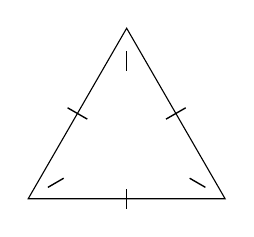
\begin{tikzpicture} [scale = 0.5, baseline=0.9cm]
                    % Draw the triangle
                    \coordinate (O) at (0,0);
                    \coordinate (A) at (5,0);
                    \coordinate (B) at (2.5,4.33);
                    \draw (O) -- (A) -- (B) -- cycle;
                    %%%
                    %Draw the line tick marks
                    \draw [line width = 0.5 pt] (2.5,-0.25) -- (2.5,0.25);
                    \draw [line width = 0.5 pt] (1.5,2.021) -- (1,2.309);
                    \draw [line width = 0.5 pt] (4,2.309) -- (3.5,2.021);
                    %%%
                    %Draw the angles
                    \tkzMarkAngle [size=0.8cm](B,A,O)
                    \tkzMarkAngle [size=0.8cm](A,O,B)
                    \tkzMarkAngle [size=0.8cm](O,B,A)
                    %%%
                    %Tick the Angles
                    \draw [line width = 0.5 pt] (2.5,3.25) -- (2.5,3.75);
                    \draw [line width = 0.5 pt] (4.5,0.288675) -- (4.1,0.52);
                    \draw [line width = 0.5 pt] (0.5,0.288) -- (0.9,0.52);
                    %%%
                \end{tikzpicture}
                &
                \textbf{Equilateral} Triangle
                & 3 Equal Sides, 3 Equal Angles \\
                \hline

                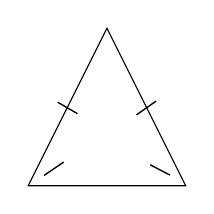
\begin{tikzpicture} [scale = 0.5]
                    %Draw the triangle
                    \coordinate (O) at (0,0);
                    \coordinate (A) at (2,4);
                    \coordinate (B) at (4,0);
                    \draw (O) -- (A) -- (B) -- cycle;
                    %%%
                    %Draw line tick marks
                    \draw [line width = 0.5 pt] (1.25,1.83) -- (0.75,2.12);
                    \draw [line width = 0.5 pt] (3.25,2.15) -- (2.75,1.8);
                    %%%
                    %Draw the angles
                    \tkzMarkAngle [size=0.8cm](B,O,A)
                    \tkzMarkAngle [size=0.8cm](A,B,O)
                    %%%
                    %Draw angle ticks
                    \draw [line width = 0.5 pt] (0.4,0.26) -- (0.9,0.6);
                    \draw [line width = 0.5 pt] (3.6,0.27) -- (3.1,0.53);
                \end{tikzpicture}
                &
                \textbf{Isosceles} Triangle & 2 Equal Sides, 2 Equal Angles \\
                \hline
                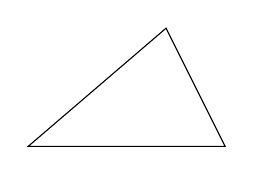
\begin{tikzpicture} [scale=0.5]
                    %Draw triangle
                    \coordinate (O) at (0,0);
                    \coordinate (A) at (3.5,3);
                    \coordinate (B) at (5,0);
                    \draw (O) -- (A) -- (B) -- cycle;
                \end{tikzpicture}
                & \textbf{Scalene} Triangle & No Equal Sides, No Equal Angles \\
                \hline
                %%%
                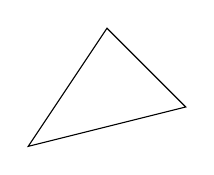
\begin{tikzpicture} [scale=0.5]
                    %Draw triangle
                    \coordinate (O) at (0,0);
                    \coordinate (A) at (2,3);
                    \coordinate (B) at (4,1);
                    \draw (O) -- (A) -- (B) -- cycle;
                    %%%
                    %Draw angles
                    \tkzMarkAngle [size=0.8cm](O,A,B)
                    \tkzMarkAngle [size=0.8cm](B,O,A)
                    \tkzMarkAngle [size=0.8cm](A,B,O)
                \end{tikzpicture}
                & \textbf{Acute} Triangle & All angles are less than $90^\circ$ \\
                \hline
                %%%
                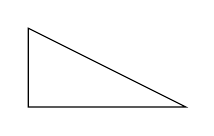
\begin{tikzpicture} [scale=0.5]
                    %Draw triangle
                    \coordinate (O) at (0,0);
                    \coordinate (A) at (0,2);
                    \coordinate (B) at (4,0);
                    \draw (O) -- (A) -- (B) -- cycle;
                    %%%
                    %Draw angles
                    \tkzMarkAngle [size=0.8cm](O,A,B)
                    \tkzMarkRightAngle [size=0.5](B,O,A)
                    \tkzMarkAngle [size=0.8cm](A,B,O)
                \end{tikzpicture}
                & \textbf{Right} Triangle & Has a right angle \\
                \hline
                %%%
                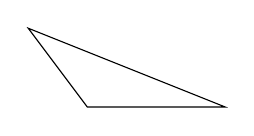
\begin{tikzpicture} [scale=0.5]
                    %Draw triangle
                    \coordinate (A) at (0,2);
                    \coordinate (B) at (1.5,0);
                    \coordinate (C) at (5,0);
                    \draw (A) -- (B) -- (C) -- cycle;
                    %%%
                    %Draw angle
                    \tkzMarkAngle [size=0.5cm](C,B,A)
                \end{tikzpicture}
                & \textbf{Obtuse} Triangle & Has an obtuse angle \\
                \hline
                %%%
                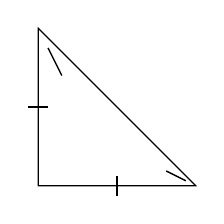
\begin{tikzpicture}[scale=0.5]
                    %Draw triangle
                    \coordinate (O) at (0,0);
                    \coordinate (A) at (4,0);
                    \coordinate (B) at (0,4);
                    \draw (O) -- (A) -- (B) -- cycle;
                    %%%
                    %Draw line ticks
                    \draw[line width=0.5 pt](2,-0.25) -- (2,0.25);
                    \draw [line width = 0.5 pt] (-0.25,2) -- (0.25,2);
                    %%%
                    %Draw angles
                    \tkzMarkAngle [size=0.5cm](O,B,A);
                    \tkzMarkAngle [size=0.5cm](B,A,O);
                    \tkzMarkRightAngle [size=0.5](B,O,A);
                    %%%
                    %Draw angle ticks
                    \draw [line width = 0.5 pt] (3.75,0.125) -- (3.25,0.375);
                    \draw [line width = 0.5 pt] (0.25,3.5) -- (0.6,2.8);
                \end{tikzpicture}
                & \textbf{Right Isosceles} Triangle
                & Has a right angle and two equal angles \\
                \hline
            \end{tabular}
        \end{center}



    \subsection{Special Triangles}
        \textbf{The $30^\circ-60^\circ-90^\circ$ Triangle}: \\

        \begin{center}
            \begin{tikzpicture} [scale=0.75]
                %Draw triangle and label sides
                \coordinate (O) at (0,0);
                \coordinate (A) at (0,2);
                \coordinate (B) at (3.4641,0);
                \draw (A) -- (O) node[midway,left] {$a$}
                -- (B) node[midway,below] {$a\sqrt{3}$}
                -- (A) node[midway,right] {$2a$}
                %%%
                %Angles // Scale not working need to edit later
                \tkzMarkAngle (A,B,O)
                \tkzMarkAngle (O,A,B)
                \tkzMarkRightAngle (A,O,B)
            \end{tikzpicture}
        \end{center}

        \noindent \textbf{The $45^\circ-45^\circ-90^\circ$ Triangle} \\

        \begin{center}
            \begin{tikzpicture} [scale=0.75]
                %Triangle
                \coordinate (O) at (0,0);
                \coordinate (A) at (0,3);
                \coordinate (B) at (3,0);
                \draw (A) -- (O) node[midway,left] {$a$}
                -- (B) node[midway,below] {$a$}
                -- (A) node[midway,right] {$a\sqrt{2}$}
                %%%
                %Angles
                \tkzMarkAngle (A,B,O)
                \tkzMarkAngle (O,A,B)
                \tkzMarkRightAngle (A,O,B)
            \end{tikzpicture}
        \end{center}



    \subsection{Triangle Formulas and Theorems}
        The \textbf{perimeter} or distance around the triangle, is given by adding up the lengths
        of the sides. Let $b$ and $h$ be the base and height of a triangle, respectively. Then, \\

        \noindent \color{purple} \textbf{Area of a Triangle:} \color{black}

        \begin{equation*}
            A=\frac{bh}{2}
        \end{equation*}

        \begin{center}
            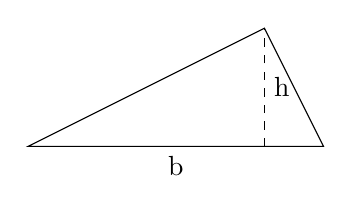
\begin{tikzpicture} [scale = 0.75]
                %Draw triangle and base
                \coordinate (O) at (0,0);
                \coordinate (A) at (4,2);
                \coordinate (B) at (5,0);
                \coordinate (C) at (4,0);
                \draw (O) -- node [midway, below] {b} (B) -- (A) -- cycle;
                %%%
                %Draw height
                \draw [dashed] (4,0) --(4,2) node [midway, right] {h};
                %%%
                %Draw right angle
                \tkzMarkRightAngle [size=0.3](B,C,A)
            \end{tikzpicture}
        \end{center}

        \noindent \color{purple} \textbf{Heron's Formula} \color{black} states that if $a,b,$ and
        $c$ are the sides of a triangle and $s$ is the triangle's \textbf{semiperimeter}, or half
        the perimeter, then the area of a triangle is given by \\

        \begin{equation*}
            A = \sqrt{s(s-a)(s-b)(s-c}
        \end{equation*}

        \noindent \color{purple} \textbf{The Pythagorean Theorem:} \color{black} for any right
        triangle with sides $a,b,c$,$c$ being the hypotenuse, \\

        \begin{equation*}
            a^2 + b^2 = c^2
        \end{equation*}

        \noindent $3,4,5$ and $5,12,13$ are some special Pythagorean numbers, called
        \textbf{Pythagorean Triples} due to their properties as integers. \\

        \noindent The \color{purple} \textbf{Triangle Inequality Theorem} \color{black} states
        that if a figure is a triangle then the sum of the lengths of any two sides is greater
        than the length of the third side. The contrapositive of this theorem also holds.

        \noindent The angle between two intersecting lines, where $m_1$ and $m_2$ are the slopes
        of the lines, is given by \\

        \begin{equation*}
            \theta = \arctan{\left|\frac{m_2-m_1}{1+m_2m_1}\right|}
        \end{equation*}



    \subsection{Construction with Triangles}
        A \textbf{median} of a triangle is a segment from a vertex to the midpoint of the opposite
        side. The \textbf{centroid} is the point at which the three medians of a triangle intersect
        and is also the centre of mass of the triangle. The \color{purple} \textbf{Centroid Theorem}
        \color{black} states that the centroid is located $\frac{2}{3}$ of the distance from each
        vertex to the midpoint of the opposite side. \\

        \begin{figure} [hbt!]
            \centering
            \includegraphics[scale = 0.075] {Resources/Unit2Triangles/centroid.PNG}
            \caption*{Medians and Centroid of a Triangle}
        \end{figure}

        \noindent An \textbf{altitude} of a triangle is a segment from a vertex constructed
        perpendicular to the opposite side. The \textbf{orthocenter} is the point at which the
        three altitudes of a triangle meet.

        \begin{figure} [hbt!]
            \centering
            \includegraphics[scale = 0.08] {Resources/Unit2Triangles/orthocenter.PNG}
            \caption*{Altitudes and Orthocenter of a Triangle}
        \end{figure}

        \noindent The \textbf{incircle} is also known as the inscribed circle. The center of
        this circle is called the \textbf{incenter} and is equidistant from all sides of the
        triangle. \\

        \begin{figure} [hbt!]
            \centering
            \includegraphics[scale = 0.75] {Resources/Unit2Triangles/incircle.jpg}
            \caption*{Incircle}
        \end{figure}

        \noindent The \textbf{circumcircle} is also known as the circumscribed circle. \\
        \begin{figure} [hbt!]
            \centering
            \includegraphics[scale = 0.75] {Resources/Unit2Triangles/circumcircle.PNG}
            \caption*{Circumcircle}
        \end{figure}



    \subsection{Congruent and Similar Triangles}
        \color{purple} \textbf{The 5 Congruency Postulates:} \color{black} \\

        \noindent \color{purple}\textbf{1. SSS (Side, Side, Side)} \color{black}\\
        \noindent If two triangles share three equal sides then the two triangles are congruent. \\

        \noindent \color{purple}\textbf{2. SAS (Side, Angle, Side)}\color{black} \\
        \noindent If two triangles share two equal sides and an equal angle between said sides
        then the two triangles are congruent. \\

        \noindent \color{purple}\textbf{3. ASA (Angle, Side, Angle)}\color{black} \\
        \noindent If two triangles share two equal angles and an equal side between said angles
        then the two triangles are congruent. \\

        \noindent \color{purple}\textbf{4. AAS (Angle, Angle, Side)}\color{black} \\
        \noindent If two triangles share two equal angles and one equal side all consecutively,
        then the two triangles are congruent. \\

        \noindent \color{purple}\textbf{5. HL (Hypotenuse, Leg)}\color{black} \\
        \noindent If two triangles share the same hypotenuse and any one of the other legs,
        then the two triangles are congruent. \\

        \noindent Similar triangles have proportional corresponding sides. For example, \\

        \begin{figure} [hbt!]
            \centering
            \includegraphics[scale = 0.6] {Resources/Unit2Triangles/sim1.PNG}
            \caption*{$\frac{AD}{DB}=\frac{EC}{BE}$}
        \end{figure}

        \noindent and \\

        \begin{figure} [hbt!]
            \centering
            \includegraphics[scale = 0.8] {Resources/Unit2Triangles/sim2.PNG}
            \caption*{$\frac{AD}{DC}=\frac{AB}{BC}$}
        \end{figure}



    \subsection{The Laws of Sine and Cosine}
        For any angles $A$,$B$, and $C$, the following definitions hold true.

        \begin{center}
            \begin{tabular}{ccc}
                $\sin A = \frac{a}{c}$
                & $\cos A = \frac{b}{c}$
                & $\tan A = \frac{a}{b}$ \\
                $\csc A = \frac{c}{a}$
                & $\sec A = \frac{c}{b}$
                & $\cot A = \frac{b}{a}$\\\\
                $\sin B = \frac{b}{c}$
                & $\cos B = \frac{a}{c}$
                & $\tan B = \frac{b}{a}$
            \end{tabular}
        \end{center}

        \begin{figure} [h]
            \centering
            \includegraphics [scale=0.4] {Resources/Unit2Triangles/Trig.fig1.png}
        \end{figure}

        \noindent From the figure, it is easy to tell that $\sin A$ and $\csc A$, $\cos A$ and
        $\sec A$, and $\tan A$ and $\cot A$ are reciprocal functions. Hence, it is usually easier
        to just work with $\sin A$, $\cos A$, and $\tan A$ Additionally,

        \begin{center}
            \begin{tabular}{ccc}
                $\frac{\sin A}{\cos A}=\tan A$
                & and &
                $\frac{\cos A}{\sin A}=\cot A$
            \end{tabular}
        \end{center}

        \noindent \color{purple} \textbf{The Law of Sines}:  \color{black}

        \begin{equation*}
            \frac{a}{\sin{A}} = \frac{b}{\sin{B}} = \frac{c}{\sin{C}}
        \end{equation*} \\

        \noindent and

        \begin{equation*}
            \frac{\sin{A}}{a} = \frac{\sin{B}}{b} = \frac{\sin{C}}{c}
        \end{equation*}

        \begin{center}
            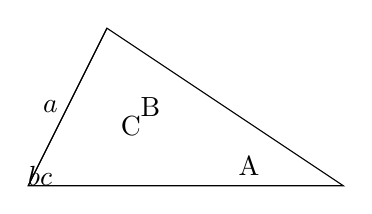
\begin{tikzpicture} [scale=1]
                %Draw triangle
                \coordinate (O) at (0,0);
                \coordinate (A) at (1,2);
                \coordinate (B) at (4,0);
                \draw (O) -- (A) -- (B) -- cycle;
                %Side markings
                \draw (A) -- (O) node[midway,left] {$a$};
                -- (B) node[midway,below] {$b$};
                -- (A) node[midway,right] {$c$};
                %Angles
                \tkzMarkAngle [size=0.8cm](O,A,B);
                \tkzMarkAngle [size=0.8cm](B,O,A);
                \tkzMarkAngle [size=0.8cm](A,B,O);
                %Angle markings \\Need to fix instead of brute forcing anchor points
                \draw (1,1) node[below] {C};
                \draw (1,1) node[below, right] {B};
                \draw (2.5,0) node[left, above] {A};
            \end{tikzpicture}
        \end{center}

        \noindent \color{purple} \textbf{The Law of Cosines:} \color{black} \\

        \begin{equation*}
            a^2 = b^2 + c^2 -2bc \cos{A}
        \end{equation*}

        \noindent and

        \begin{equation*}
            \cos{A}=\frac{b^2+c^2-a^2}{2bc}
        \end{equation*}



    \subsection{Ceva's Theorem}
        A \textbf{cevian} is a line that intersects both a triangle's vertex and the side
        opposite to said vertex. Medians and angle bisectors are special cases of cevians.
        \color{purple} \textbf{Ceva's Theorem} \color{black} is a criterion for the concurrence
        of cevians in a triangle. \textbf{Concurrence} means that several lines or curves
        intersect at a certain point. \\

        \noindent It states that if $ABC$ is a triangle and $D,E,F$ are all points on
        $\overline{BC},\overline{CA},\overline{AB}$, respectively, then $\overline{AD},
        \overline{BE},\overline{CF}$ are concurrent if and only if \\

        \begin{equation*}
            \frac{BD}{DC}\cdot\frac{CE}{EA}\cdot\frac{AF}{FB}=1
        \end{equation*}

        \noindent Since the reciprocal of 1 is 1, the reciprocals of the ratios also have a
        product of 1. \\

        \begin{figure} [hbt!]
            \centering
            \includegraphics[scale=0.75]{Resources/Unit2Triangles/ceva.PNG}
        \end{figure}



    \pagebreak
    \subsection{Menelaus' Theorem}
        \color{purple} \textbf{Menelaus' Theorem} \color{black} describes the collinearity of
        points on each of the three sides of a triangle. It states that if $\overline{PQ}$
        intersects $\overline{AB}$ on $\triangle ABC$ where $P$ is on $\overline{BC}$, $Q$ is
        the extension of $\overline{AC}$, and $R$ is on the intersection of $\overline{PQ}$ and
        $\overline{AB}$, then \\

        \begin{equation*}
            \frac{PB}{CP}\cdot\frac{QC}{QA}\cdot\frac{AR}{RB}=1
        \end{equation*}

        \begin{figure} [hbt!]
            \centering
            \includegraphics[scale=0.75]{Resources/Unit2Triangles/menelaus.PNG}
        \end{figure}